%
% proposal.tex
%
% Dissertation Proposal Template.
% School of Computing
% Clemson University
%
\documentclass[10pt]{ClemsonProposal}


% This is nice for source code listings
% \usepackage{listings}

% This is needed to include figures
% \usepackage{graphicx}

% Use any additional packages you might need
\let\oldbibitem\bibitem
\def\bibitem{\vfill\oldbibitem}

\usepackage{booktabs} % For formal tables
\usepackage{epsfig,endnotes,subcaption,url}
\usepackage{flushend}
\usepackage{amsmath}
%\usepackage{subfigure}
\usepackage{float}
\usepackage{pifont}
%\usepackage{subfig}

\usepackage{multirow}
\usepackage{pifont}% http://ctan.org/pkg/pifont
\newcommand{\cmark}{\ding{51}}%
\newcommand{\xmark}{\ding{55}}%

%
% Give values to the variables used in this document
%
\title{Using Endpoint Asymmetry to Detect and Correct Network Performance Issues in CDNs}
\department{Electrical Engineering and Computer Science}
\documenttype{Dissertation Proposal}
\major{Computer Science}
\proposalday{24}
\proposalmonth{September}
\proposalyear{2018}
\author{Marc Anthony Warrior}
\committeechair{Aleksandar Kuzmanovic}
\committeememberone{Fabi\'an Bustamante}
\committeemembertwo{Peter Dinda}
\committeememberthree{Theophilus A. Benson}

% Just in case you have more then 3 committee members
% \committeememberfour{Member4 Name}
% \committeememberfive{Member5 Name}
% \committeemembersix{Member6 Name}


%
% PDF Setup -- You should not need to change this
%
\hypersetup{	
    colorlinks,
    linkcolor={black},
    citecolor={black},
    filecolor={black},
    urlcolor={black},
    pdftitle={\thetitle},
    pdfauthor={\theauthor},
    pdfsubject={\thedocumenttype},
    pdfstartpage={1}
}


%
% User-specified command definitions/redefinitions
%
\newcommand{\cplusplus}{{\rm C\raise.5ex\hbox{\small ++}}}


\begin{document}
%   ==========================================================================
%   Begin front matter (pages are numbered with roman numerals)
%   ==========================================================================
    \begin{frontmatter}
        \maketitle
		\tableofcontents
        \newpage

        % Generate the abstract
        \begin{abstract}

``Do you see what I see?'' The vastness of today's Internet creates an intuitive
but often overlooked phenomenon: not everyone is exposed to the same web
resources. Even across the set of objects embedded in a single web page, a pair of
clients with apparently similar network properties may be assigned to barely
overlapping sets of network resources to pull from. While the properties of
individual content distribution networks (CDNs) and the like are well explored,
there has been, until now, a lack of insight regarding the \emph{aggregate}
behavior of these many large networks co-existing.  

In this paper, we perform the first, deep analysis of cross-provider resource
allocation patterns and the resulting aggregate mapping of over 10,000 RIPE
Atlas clients around the world. To facilitate our research, we introduce common
network resource exposure (CNRE) - a measure of the degree to which a pair of
clients are exposed to the same network destinations as each other across a
large set of domains. We explore the implications of high and low CNRE scores,
and assess the applicability of well established network properties (country,
ASN, BGP prefix, and /24) in estimating CNRE. Our findings expose clients that
are poorly served by their current position in this aggregate mapping scheme and
highlight the existence of ``outlier'' CDNs, who allocate their resources in a
way that goes against broader Internet trends.

\end{abstract}



	\end{frontmatter}



%   ==========================================================================
%   Begin main matter (pages are numbered with arabic numerals)
%   ==========================================================================
    \doublespacing     % Text should be double spaced
    \pagestyle{fancy}  % Turn the nice header on for the rest of the document

    %
    % I use a file for every section.  Each of these corresponds to a file
    % with the specified name ending in '.tex' (e.g., introduction.tex).
    %
    \section{Introduction} \label{sect:intro}

You and the person next to you might not be using the same Internet. With
ever increasing diversity and interlinking of online services  --- content distribution networks (CDNs), cloud computing, CDN and
cloud brokers, ad brokers, load balancing, user tracking, geoIP, and more --- even the
implications
of loading a single web page are no longer straightforoard CITE. Often, failure to
recognize the whole as distinct from the sum of its parts has inhibited progress
and hampered performance in networking technology CITE. In the same way a city's
skyline cannot be anticipated by the artitect of a single  building, the
``digital skyline'' of the Internet can be neither predicted nor fully
controlled by any single entity.
However, skylines can always be \emph{observed}.

Even across a single network service, client experiences may diverge. In Figure
\ref{fig:dnsmiss}, we provide a high level illustration of how this can happen.
In subfigure \ref{fig:dns},  a client intending to connect to example.com submits a DNS query. We do not
concern the minute details of
the DNS resolution process, which is itself multi-tierd and possibly involving
cooperation from many separate stakeholders. What is important to know is that
eventually, the client's request reaches the nameserver responsible for
example.com. The nameserver uses what is often internal, proprietary
logic to decide which of example.com's network resources the client should be
connected to. In subfigure \ref{fig:mismatch}, we are reminded that this client
is not the only one access example.com. However, as illustrated,
the client's peers may not necessarily be directed to the same resource, despite
having carried out essentially the same DNS resolution process and possibly
sharing the same edge network. This potential for mismatch between clients only
grows as the number of domains considered increases --- which it will, often on
a single web page.

In this paper, we explore the complex combination of independently operating
resource allocation schemes and assess their behavior in \emph{aggregate}. To
enable our research, We introduce a new similarity measure, common network
resource exposure (CNRE), which captures the extent to which a pair of clients
are directed to the same network targets as each other across a broad set of
domains. CNRE is, to our knowledge, the first ever method to quantify
cross-provider DNS redirection patterns and their collective behavior. 

We test and assess CNRE using 302 web content hosting domains for each CNRE
calculation.  To do this, we collect latency and DNS measurements for each
domain from each of 9,024 globally distributed clients and perform over 40
million pairwise CNRE calculations between them. Our experiments 
validate common network research exposure as a useful quantity and explore its
relationship with other cilent properties.

\begin{figure*}
    \center
        \mbox{
            \begin{subfigure}[b]{0.5\linewidth}
                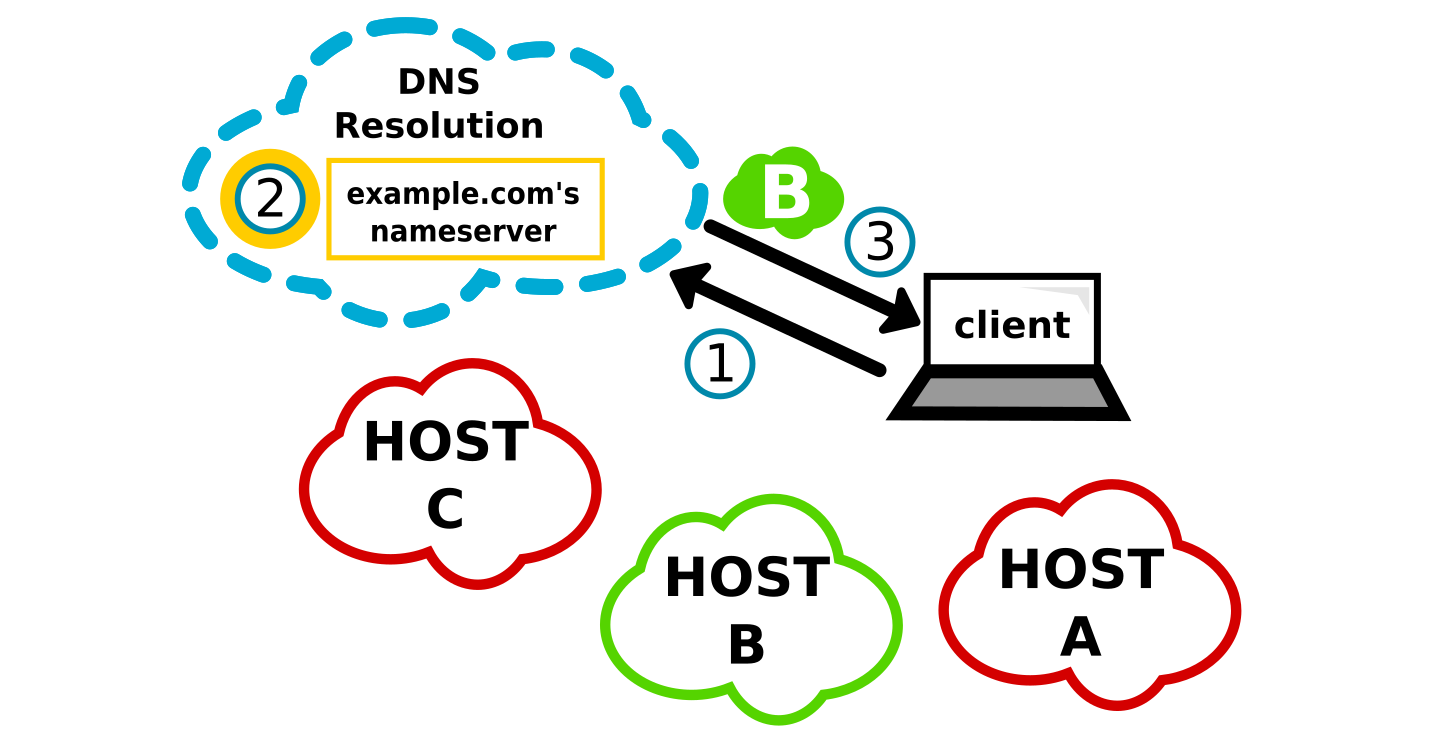
\epsfig{file=figs/dns_resolution.png, width=1\linewidth}
                \caption{\label{fig:dns}}
            \end{subfigure}
            \begin{subfigure}[b]{0.5\linewidth}
                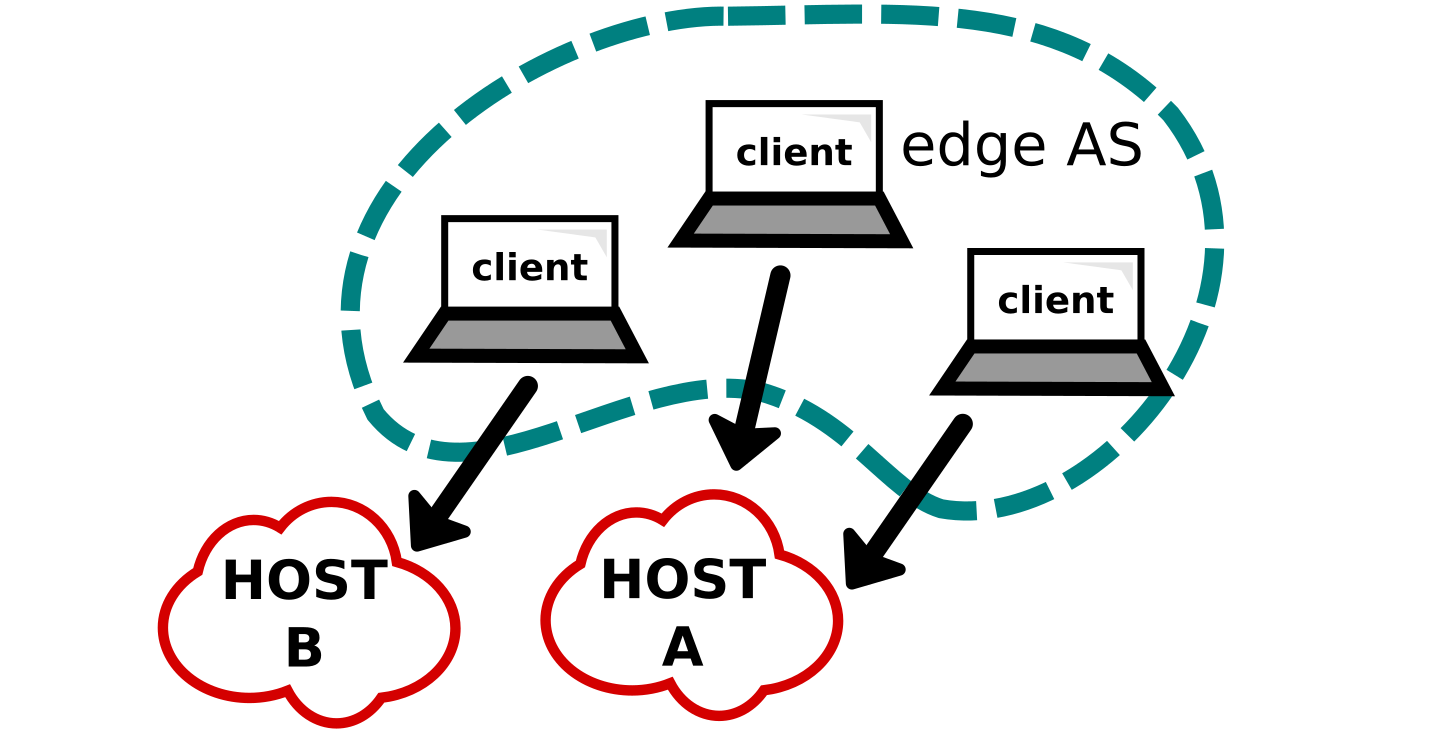
\epsfig{file=figs/client_mapping.png, width=1\linewidth}
                \caption{\label{fig:mismatch}}
            \end{subfigure}
        }
    \caption{
        Illustration of network resource allocation. Figure \ref{fig:dns} shows DNS resolution at a high level: 1)~The client deploys a DNS query for example.com. 2) This query ultimately reaches nameserver responsible for example.com and decides which of example.com's network resources should serve the client. 3) The nameserver's resource selection is returned to the client. Figure \ref{fig:mismatch} shows an example of how clients with similarly described locations may
        be directed to distinct network resources.
    }
    \ref{fig:dnsmiss}
\end{figure*}

In order to develop the Skyline model, we performed an exhaustive set of measurements to frame
client experience on a per \emph{site} basis. In this work, we capture a
snapshot of both DNS resolutions and latency measurements toward the 304 domains that appeared most
frequently in the top 2441 most popular webpages. Our measurements span over
9,000 unique
clients spread across 185 countries and 3637 autonomous systems. We performed over 52 million pairwise
comparisons with the results of these measurements to arrive at the foundation of what we have
coined the ``Skyline model". 

This paper makes the following contributions: %, including those we expect to stem from
%proposed work, which we have designated with (\emph{p})

\begin{itemize}%\parskip0pt \parsep0pt
    \item We perform a large exploration of client network performance on a per webpage level. Our
        raw results are publicly available on the RIPE Atlas platform.
    \item  We quantify the degree of misalignment between conventional grouping schemes
        and aggregate catchments.
    \item  We introduce the Skyline model, a client grouping scheme that reflects the
        extent of CNRE.
    \item  Using the Skyline model, we identify and analyze network resource islands --- 
        sets of clients with very high degrees CNRE. 
\end{itemize}

% RELATED WORK and PROBLEM FRAMING
\section{Problem Space and Related Work} \label{skyspace}

This projects aims to gain an understanding of which clients are directed to the same set of
resources across many distinct domains. Its most direct and immediate use case is influencing probe
selection in large scale Internet measurements. For researchers, likely unaware of the relatively
hidden allocation schemes of the wide array of CDN platforms and other large content distributors,
it is difficult to determine, a priori, the degree of similarity between clients. Knowledge of
whether there is a high probability that a pair of clients are being directed to altogether
different resources may be significant to their experiment design. This approach to experiment
design is in line with RIPE Atlas, one of the largest client based measurement platforms,
which maintains
an exhaustive set of tags on all of their clients in order to help researchers and network operators
filter and refine the set selected for their experiment \cite{ripe-atlas}. Further, more abstract
applications may include, but are not limited to, distributed denial of service mitigation
\cite{anycastvsddos} and CDN node deployment \cite{35590, Tariq}.

The most similar body of related work involves anycast CDN catchment analysis, which aims to
investigate the set of clients routed towards particular CDN points of presence (PoPs)
\cite{Calder2015, anycastvsddos, vdmscatchment}. Our work differs significantly in scope: to our 
knowledge, we are the first to investigate what we refer to as \emph{aggregate catchments}, the joint
behavior of many anycast CDN catchments and unicast CDN targets, spread across many content
distribution platforms. Conversely, this related body work either focuses on individual platforms or
specific services \cite{Calder2015, anycastvsddos, vdmscatchment}. 

Several authors have attempted to discover the topology of large CDN platforms through large scale
measurement studies \cite{webcart, Calder2013, benson11}. While their findings are potentially of
use in this project, their goals and contributions run parallel to what we aim to accomplish. They
seek to identify the properties and locations of CDN resources; conversely, we seek to identify the
target pools (sets of clients) of overlapping CDN resource catchments \cite{webcart, Calder2013,
benson11}. Other work close to this space investigates the performance of a particular CDN
deployment scheme \cite{ecs15sigcomm}.

    \input{thesis}
    \include{drongo}
    \documentclass[10pt, sigconf]{acmart}

\let\oldbibitem\bibitem
\def\bibitem{\vfill\oldbibitem}

\usepackage{booktabs} % For formal tables
\usepackage{epsfig,endnotes,subcaption,url}
\usepackage{flushend}


% Copyright
%\setcopyright{none}
%\setcopyright{acmcopyright}
%\setcopyright{acmlicensed}
%\setcopyright{rightsretained}
%\setcopyright{usgov}
%\setcopyright{usgovmixed}
%\setcopyright{cagov}
%\setcopyright{cagovmixed}


\begin{document}
\title[Skylines]{Skylines: Pragmatic, Perspective-Based Internet Mapping}
%\titlenote{Produces the permission block, and copyright information}
%\subtitle{Extended Abstract}

\author{Marc Anthony Warrior}
\affiliation{%
  \institution{Northwestern University}
}
\email{warrior@u.northwestern.edu}

\author{Romain Fontugne}
\affiliation{%
  \institution{IIJ Innovation Institute}
}
\email{romain@iij.ad.jp}
\author{Randy Bush}
\affiliation{%
  \institution{IIJ Innovation Institute}
}
\email{randy@psg.com}

\renewcommand{\shortauthors}{M. Warrior et al.}

\begin{abstract}

    Existing mapping systems and measures used to describe Internet location
    fail to account for complexities introduced by DNS-based content
    allocation schemes. With DNS redirection, in particular, clients residing in
    the exact same network location may potentially be served by completely
    different content sources. Likewise, distant clients may be directed to the
    same servers. The existence of such scenarios challenges the validy of
    some common assumptions about network behavior: the relationship between a
    client's network location and its ``view'' of the Internet, independent of
    performance, is neither predictable nor consistent across clients. 

    In this paper, we introduce skylines, a distance measure that describes
    variation in Internet resource allocation between clients. TODO: finish list
    of contributions

\end{abstract}

%
% The code below should be generated by the tool at
% http://dl.acm.org/ccs.cfm
% Please copy and paste the code instead of the example below. 
%

\copyrightyear{2018} 
\acmYear{2018} 
\setcopyright{acmcopyright}
\acmConference[IMIC '18]{IMC '18: ACM Internet Measurement Conference 2018,
October 31--November 2, 2018}
\acmBooktitle{IMC '18: ACM Internet Measurement Conference 2018,
October 31--November 2, 2018}
\acmPrice{15.00}
\acmDOI{0.0/0.0}
\acmISBN{0-0-0-0-0/0/0}

\begin{CCSXML}
<ccs2012>
    <concept>
        <concept_id>#.#.#</concept_id>
        <concept_desc>Networks~Application layer protocols</concept_desc>
        <concept_significance>300</concept_significance>
    </concept>
    <concept>
        <concept_id>#.#.#</concept_id>
        <concept_desc>Networks~Naming and addressing</concept_desc>
        <concept_significance>100</concept_significance>
    </concept>
    <concept>
        <concept_id>#.#.#</concept_id>
        <concept_desc>Networks~Location based services</concept_desc>
        <concept_significance>100</concept_significance>
    </concept>
</ccs2012>
\end{CCSXML}

\ccsdesc[300]{Networks~Application layer protocols}
\ccsdesc[100]{Networks~Naming and addressing}
\ccsdesc[100]{Networks~Location based services}

% We no longer use \terms command
%\terms{Theory}

\keywords{DNS, CDN, replica server, subnet}

\maketitle

\section{Background \& Motivation} \label{sect:background}
\begin{enumerate}
    \item site performance is dependent on many underlying content sources
        \begin{enumerate}
            \item for Alexa top 500: 50+ domain resolutions per site in median case, 100+ in 80th
                percentile \cite{dnssly}
            \item providers are concerned with the ``bottlenecks'' induced by
                poorly optimized external services (TODO: citations)
            \item providers are interested in coalescing connections where
                possible (TODO: citations; spdy, quic)
        \end{enumerate}
    \item existing measurement and optization efforts tend to focus on
        individual services, often neglecting the complexity of page load times
        and likelihood of external bottlenecks
        \begin{enumerate}
            \item (CDN) resource allocation and mapping algorithm / analysis (TODO: cite
                examples)
            \item client location algorithms and analysis (TODO: cite examples)
        \end{enumerate}
\end{enumerate}

\section{Overview / Goal}
Given that no provider is an island (see \ref{sect:background}), we need to know
how client to sever mapping schemes work \emph{together}, across providers.

Potential applications and insights:
\begin{enumerate}
    \item services may be able to make better decisions about how to allocate
        and/or share infrastructure with other providers
    \item services can better identify potential external sources of outlier behavior
    \item researchers can make more informed decisions in large scale internet
        experiment design and analysis (particularly regarding client grouping)
\end{enumerate}

\section{Approach}
\begin{enumerate}
    \item we DNS resolution to determine mapping schemes, as DNS redirection is
        both widely used and publicly exposed
        \begin{enumerate}
            \item we first identify sites that use DNS redirection 
            \item we then determine the granularity with which sites use DNS
                redirection.
                \begin{enumerate}
                    \item if a site has few unique IPs, it may be using anycast,
                        in which case the details of their mapping scheme is
                        potentially unexposed to the public 
                    \item alternatively, a service with few IPs might actually
                        have few resource locations. There
                        is not much to analyze regarding such a service in the
                        context of this paper, as such a small distribution
                        would inherently have very little overlap with any
                        large scale mapping schemes.
                \end{enumerate}
            \item next, we extract general properties and patterns from the
                remaining, sufficiently granular dataset. We'll use these
                findings to form our distance measure, which will drive the rest
                of our analysis
        \end{enumerate}
    \item we form a distance measure, describing the degree of similarity
        between two clients in terms of the set of web resources they are
        exposed to (in the context of DNS redirection)
    \item ...
\end{enumerate}

\clearpage

\bibliographystyle{ACM-Reference-Format}
\bibliography{skylines} 

\end{document}

    \include{proposed_work}



%   ==========================================================================
%   Wrap up the document with the Bibliography (looks for the specified .bib)
%   ==========================================================================
    \makebibliography{bibliography}
\end{document}
